\documentclass[11pt]{article}
\usepackage[a4paper,margin=25mm]{geometry}
\usepackage[T1]{fontenc}
\usepackage{amsmath,amssymb,amsthm}
\usepackage{tikz}
\usepackage{lmodern}
\usepackage[hidelinks]{hyperref}

\newtheorem*{drc}{Theorem 1.7.5}
\newcommand{\ex}{\operatorname{ex}}

\title{Dependent random choice}
\author{Yufei Zhao\\[2pt]
\small Section 1.7 of \emph{Graph Theory and Additive Combinatorics},
author manuscript updated 2024-06-18}
\date{Printed pages 34--35 (physical pages 50--51)}

\begin{document}
\maketitle

% BEGIN CONTEXT ZHAO:I1_7
\noindent\textbf{Source and scope.}
This is Theorem 1.7.5 of Yufei Zhao, \emph{Graph Theory and Additive
Combinatorics}, author manuscript updated 2024-06-18, printed pages 34--35
(physical pages 50--51 of the author PDF), together with its printed proof and
the printed remark on parameters that stands between the statement and the
proof. The statement and the proof are reproduced in full; nothing is added,
shortened or repaired.

The theorem is stated inside Section 1.7, which introduces the dependent random
choice technique. The one schematic in the proof is redrawn in \TeX{} from the
printed drawing: hosts $u_1,\dots,u_t$ on top, every displayed host joined to
every displayed vertex of the common neighbourhood $A$ below, with $A$ shown as
a shaded strip. The drawing is schematic in the source as well, and no
additional hypothesis is read from it.

One printed detail is kept literally rather than normalised: the convexity
display prints the averaging sum with the subscript $v\in V$ (not $v\in V(G)$).
It is reproduced as printed and is recorded in the transcription fidelity
review.

Permission: the author makes the manuscript publicly available, but permission
to redistribute edited excerpts is not established. This reader is a private
working copy inside the corpus maintenance workspace and is not published.

% END CONTEXT ZHAO:I1_7

% BEGIN PRIMARY STATEMENT ZHAO:I1_7
\begin{drc}[Dependent random choice]
Let $n,r,m,t$ be positive integers and $\alpha>0$. Then every graph $G$ with
$n$ vertices and at least $\alpha n^2/2$ edges contains a vertex subset $U$
with
\[
  |U| \;\ge\; n\alpha^{t}-\binom{n}{r}\Bigl(\frac{m}{n}\Bigr)^{t}
\]
such that every $r$-element subset $S$ of $U$ has more than $m$ common
neighbors in $G$.
\end{drc}
% END PRIMARY STATEMENT ZHAO:I1_7

% BEGIN PRIMARY PROOF ZHAO:I1_7
\noindent\emph{Remark 1.7.6 (Parameters).} In the theorem statement, $t$ is an
auxiliary parameter that does not appear in the conclusion. While one can
optimize for $t$, it is instructive and convenient to leave it as is. The
theorem is generally applied to graphs with at least $n^{2-c}$ edges, for some
small $c>0$, and we can play with the parameters to get $|U|$ and $m$ both
large as desired.

\begin{proof}
We say that an $r$-element subset of $V(G)$ is ``bad'' if it has at most $m$
common neighbors in $G$.

Let $u_1,\dots,u_t$ be vertices chosen uniformly and independently at random
from $V(G)$. (These vertices are chosen ``with replacement,'' i.e., they can
repeat.) Let $A$ be their common neighborhood. (Keep in mind that
$u_1,\dots,u_t,A$ are random. It may be a bit confusing in this proof to see
what is random and what is not.)

\begin{center}
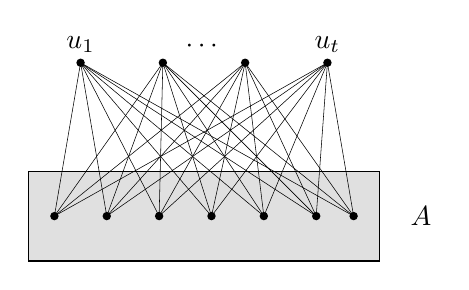
\begin{tikzpicture}[scale=0.95]
  % four top markers, labelled u_1, then the ellipsis, then u_t, as printed
  \foreach \x in {0,1.1,2.2,3.3} { \fill (\x,1.7) circle (1.6pt); }
  \node[above] at (0,1.7) {$u_1$};
  \node[above] at (1.65,1.7) {$\cdots$};
  \node[above] at (3.3,1.7) {$u_t$};
  % shaded common neighbourhood strip holding seven vertices
  \fill[black!12] (-0.7,-0.95) rectangle (4.0,0.25);
  \draw (-0.7,-0.95) rectangle (4.0,0.25);
  \node at (4.55,-0.35) {$A$};
  \foreach \x in {-0.35,0.35,1.05,1.75,2.45,3.15,3.65} {
    \fill (\x,-0.35) circle (1.6pt);
  }
  % every displayed top marker joined to every displayed vertex of A
  \foreach \u in {0,1.1,2.2,3.3} {
    \foreach \x in {-0.35,0.35,1.05,1.75,2.45,3.15,3.65} {
      \draw[very thin] (\u,1.7) -- (\x,-0.35);
    }
  }
\end{tikzpicture}
\end{center}

Each fixed vertex $v\in V(G)$ has probability $(\deg(v)/n)^{t}$ of being
adjacent to all of $u_1,\dots,u_t$, and so, by linearity of expectations and
convexity,
\[
  \mathbb{E}|A|
  =\sum_{v\in V(G)}\mathbb{P}(v\in A)
  =\sum_{v\in V(G)}\Bigl(\frac{\deg(v)}{n}\Bigr)^{t}
  \;\ge\; n\Bigl(\frac{1}{n}\sum_{v\in V}\frac{\deg(v)}{n}\Bigr)^{t}
  \;\ge\; n\alpha^{t}.
\]

For any fixed $R\subseteq V(G)$,
\[
  \mathbb{P}(R\subseteq A)
  =\mathbb{P}(R\text{ is complete to }u_1,\dots,u_t)
  =\Bigl(\frac{\#\text{ common neighbors of }R}{n}\Bigr)^{t}.
\]
If $R$ is a bad $r$-vertex subset, then it has at most $m$ common neighbors,
and so
\[
  \mathbb{P}(R\subseteq A)\;\le\;\Bigl(\frac{m}{n}\Bigr)^{t}.
\]
Therefore, summing over all $\binom{n}{r}$ possible $r$-vertex subsets
$R\subseteq V(G)$, by linearity of expectation,
\[
  \mathbb{E}[\text{the number of bad }r\text{-vertex subsets of }A]
  \;\le\;\binom{n}{r}\Bigl(\frac{m}{n}\Bigr)^{t}.
\]
Let $U$ be obtained from $A$ by deleting an element from each bad $r$-vertex
subset. So, $U$ has no bad $r$-vertex subsets. Also,
\[
  \mathbb{E}|U|
  \;\ge\;\mathbb{E}|A|-\mathbb{E}[\text{the number of bad }r\text{-vertex
  subsets of }A]
  \;\ge\; n\alpha^{t}-\binom{n}{r}\Bigl(\frac{m}{n}\Bigr)^{t}.
\]
Thus, there exists some $U$ with at least this size, with the property that all
its $r$-vertex subsets have more than $m$ common neighbors.
\end{proof}
% END PRIMARY PROOF ZHAO:I1_7

\end{document}
